% Design 
%!TEX root = ../Project.tex
\section{Design}

\subsection{Methodologies}
\label{sub:methodologies}
The Model, View, Controller (MVC) design paradigm was chosen to be used to structure the project. The MVC design patten has many benefits as discussed below.  

%TODO

\subsection{Engine}
The main considerations  for the engine was to it made it configureable as possible. To achieve this everything was designed in term of interfaces, which allowed the particular implementation to be changed. The objects themselves were loaded from their serialised form on disk. 

\subsubsection{Data Format}
XMl was chosen as the data format for this project. The main reason is that it is human readable, this allow me to create and test the data format before the editor was created.

The data was design to be extendable, as well as provide implementations of the various assets the advance user can specify their own custom classes.
\begin{lst:weapon}[caption=Example of Custom weapon, label=lst:weapon]
<weapon class="custom.customWeapon" uuid="0f0dee33">
	<name>Longicolnis</name>
</weapon>
\end{lst:weapon}
Listing \ref{lst:weapon} shows how a custom weapon can be used. The \texttt{class} attribute is  the full quified name of the class. The only thing the user has to use their class is to add a jar with class in it to the \texttt{classpath} of the game. 

\subsubsection{XML schema}

XML schema is a way of validating a  xml document. A schema was produced for each serialised object\footnote{in the \texttt{schemas} directory}. 
The main use of this was for testing of the hand written xml I used before the editor was created. It also helped ensure that the xml produced by the editor was correct.  

\subsection{Game Progression}
\begin{figure}[htbp]
	\centering
		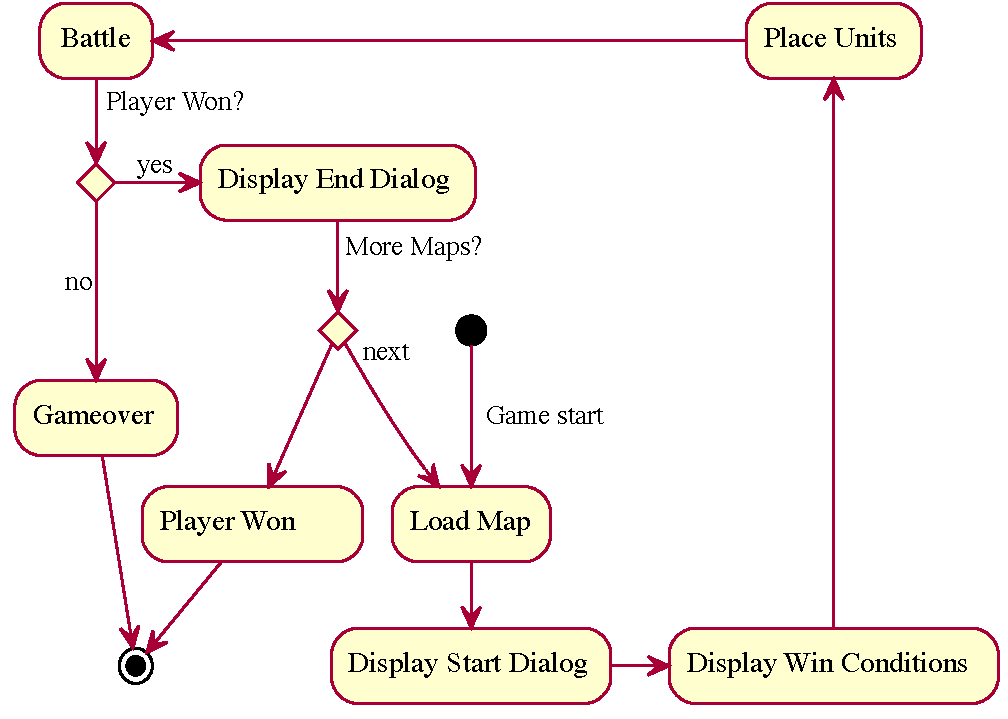
\includegraphics[height=3in]{figures/game.pdf}
	\caption{Activity diagram which a high level of overview of the engine}
	\label{fig:figures_game}
\end{figure}

Figure \ref{fig:figures_game} shows the overview of how the created game progress.  Each game has a number of maps where a battle take place. After the map is loaded any relanent dialog is displayed, along with winning conditions. The player's units are then placed are the map, and the battle starts\footnote{While the engine support allowing the user's to choose where the their units are placed, the GUI does not due to time constraints. The editor does support specify the starting location for the player's units.}. If the player's loses the battle, a gameover screen is shown and the game ends. In contrast if the player wins he/she advances to the next map, if there is one.    

\subsection{Gui}

\subsubsection{Tilemap}
\label{sub:tilemap}

There were two main choices for the isometric tilemap, a ``Diamond'' map or a  ``Staggered'' map \cite{isometric_game_programming}, examples of both are shown below in figure \ref{fig:tilemap0}. Prototypes of each map type were and the following was found.  

The ``Staggered'' was the first to be considered and the following advantages:
\begin{itemize}
	\item The map fill up the screen with very little wasted space, so the user can more of what happing on the map. 
\end{itemize}

The ``Diamond'' map was chosen for the following reasons:
\begin{itemize}
	\item ``Diamond'' map look more astiricly pleasing  then ``Staggered'' maps because it has no ragged edges.
	\item  If the map is large enough it will the whole screen negating ``Staggered'' map advantage.
	\item  Simpler to think about, since a `Diamond' map is just a rectangular map rotated.
\end{itemize}


\def\tilemapSize{5in}
\begin{figure}[htbp]
	\begin{center}

	\subfigure[Diamond Map]{
		\label{fig:tilemap1} 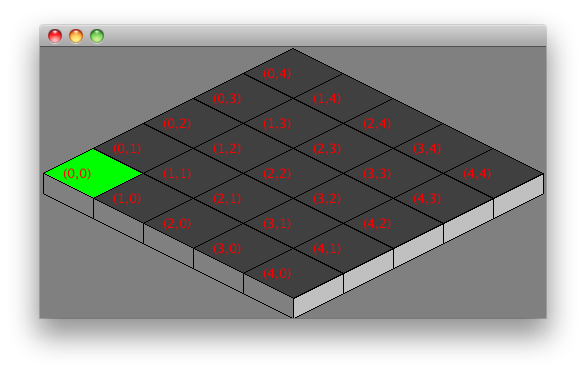
\includegraphics[width=\tilemapSize]{figures/tilemap1.png}} 
	\subfigure[Staggered Map]{
		\label{fig:tilemap2} 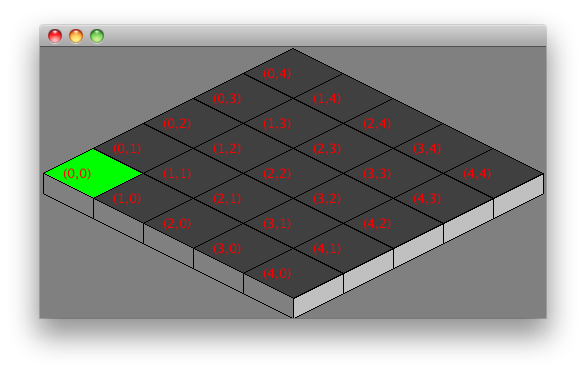
\includegraphics[width=\tilemapSize]{figures/tilemap2.png}} 
	\caption{\label{fig:tilemap0} The two main types of isometric tilemaps}
	\end{center}
\end{figure}

\clearpage
\subsubsection{Unit}
\label{ssub:unit}
I design the unit actions as a finite state machine as show in figure \ref{fig:figures_unit}.  The 

\begin{figure}[h]
	\centering
		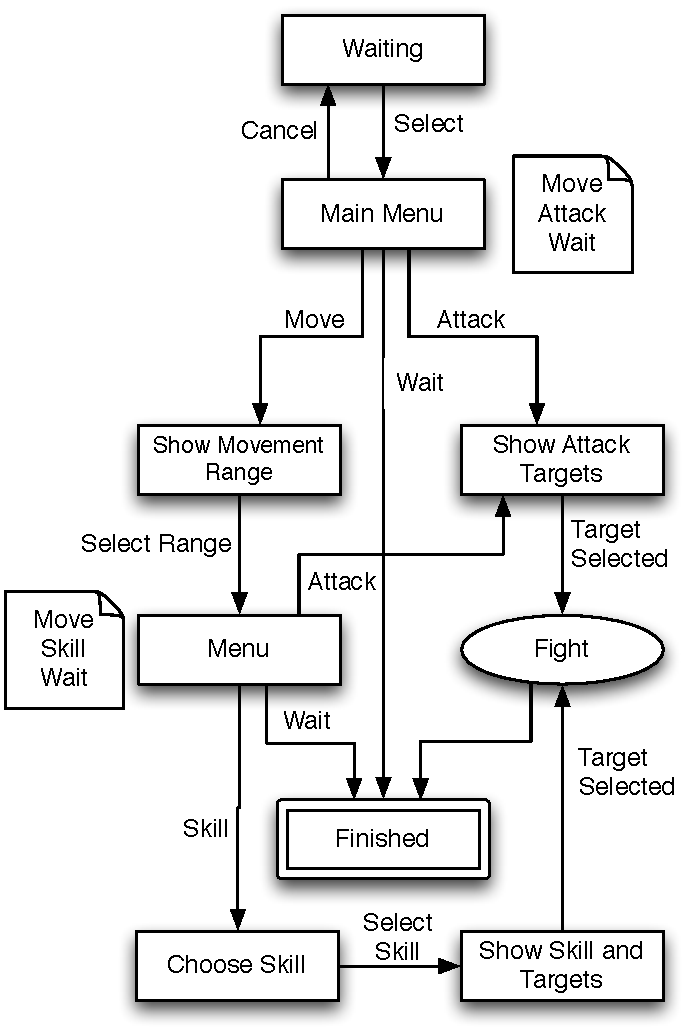
\includegraphics[width=4in]{figures/unit.pdf}
	\caption{The State diagram of a single turn of a player's unit}
	\label{fig:figures_unit}
\end{figure}

% add pics